\documentclass[11pt,compress,t,notes=noshow, xcolor=table]{beamer}
\usepackage[]{graphicx}\usepackage[]{color}
% maxwidth is the original width if it is less than linewidth
% otherwise use linewidth (to make sure the graphics do not exceed the margin)
\makeatletter
\def\maxwidth{ %
  \ifdim\Gin@nat@width>\linewidth
    \linewidth
  \else
    \Gin@nat@width
  \fi
}
\makeatother

\newcommand{\citebutton}[2]{%
\beamergotobutton{\href{#2}{#1}}%
}

\newcommand{\blu}[1]{\textcolor{blue}{#1}}
\newcommand{\org}[1]{\textcolor{orange}{#1}}
\newcommand{\ques}{\textbf{\textcolor{red}{Question:  }}}
\newcommand{\questionssofar}{\begin{frame}\frametitle{Any questions?}\end{frame}}

\newcommand\warning{%
 \makebox[1.4em][c]{%
 \makebox[0pt][c]{\raisebox{.1em}{\scriptsize!}}%
 \makebox[0pt][c]{\color{red}\normalsize$\bigtriangleup$}}}%

\definecolor{fgcolor}{rgb}{0.345, 0.345, 0.345}
\newcommand{\hlnum}[1]{\textcolor[rgb]{0.686,0.059,0.569}{#1}}%
\newcommand{\hlstr}[1]{\textcolor[rgb]{0.192,0.494,0.8}{#1}}%
\newcommand{\hlcom}[1]{\textcolor[rgb]{0.678,0.584,0.686}{\textit{#1}}}%
\newcommand{\hlopt}[1]{\textcolor[rgb]{0,0,0}{#1}}%
\newcommand{\hlstd}[1]{\textcolor[rgb]{0.345,0.345,0.345}{#1}}%
\newcommand{\hlkwa}[1]{\textcolor[rgb]{0.161,0.373,0.58}{\textbf{#1}}}%
\newcommand{\hlkwb}[1]{\textcolor[rgb]{0.69,0.353,0.396}{#1}}%
\newcommand{\hlkwc}[1]{\textcolor[rgb]{0.333,0.667,0.333}{#1}}%
\newcommand{\hlkwd}[1]{\textcolor[rgb]{0.737,0.353,0.396}{\textbf{#1}}}%
\let\hlipl\hlkwb

\usepackage{framed}
\makeatletter
\newenvironment{kframe}{%
 \def\at@end@of@kframe{}%
 \ifinner\ifhmode%
  \def\at@end@of@kframe{\end{minipage}}%
  \begin{minipage}{\columnwidth}%
 \fi\fi%
 \def\FrameCommand##1{\hskip\@totalleftmargin \hskip-\fboxsep
 \colorbox{shadecolor}{##1}\hskip-\fboxsep
     % There is no \\@totalrightmargin, so:
     \hskip-\linewidth \hskip-\@totalleftmargin \hskip\columnwidth}%
 \MakeFramed {\advance\hsize-\width
   \@totalleftmargin\z@ \linewidth\hsize
   \@setminipage}}%
 {\par\unskip\endMakeFramed%
 \at@end@of@kframe}
\makeatother

\definecolor{shadecolor}{rgb}{.97, .97, .97}
\definecolor{messagecolor}{rgb}{0, 0, 0}
\definecolor{warningcolor}{rgb}{1, 0, 1}
\definecolor{errorcolor}{rgb}{1, 0, 0}
\newenvironment{knitrout}{}{} % an empty environment to be redefined in TeX

\usepackage{alltt}
\newcommand{\SweaveOpts}[1]{}  % do not interfere with LaTeX
\newcommand{\SweaveInput}[1]{} % because they are not real TeX commands
\newcommand{\Sexpr}[1]{}       % will only be parsed by R
\newcommand{\xmark}{\ding{55}}%


\usepackage[english]{babel}
\usepackage[utf8]{inputenc}

\usepackage{dsfont}
\usepackage{verbatim}
\usepackage{amsmath}
\usepackage{amsfonts}
\usepackage{amssymb}
\usepackage{bm}
\usepackage{csquotes}
\usepackage{multirow}
\usepackage{longtable}
\usepackage{booktabs}
\usepackage{enumerate}
\usepackage[absolute,overlay]{textpos}
\usepackage{psfrag}
\usepackage{algorithm}
\usepackage{algpseudocode}
\usepackage{eqnarray}
\usepackage{arydshln}
\usepackage{tabularx}
\usepackage{placeins}
\usepackage{tikz}
\usepackage{setspace}
\usepackage{colortbl}
\usepackage{mathtools}
\usepackage{wrapfig}
\usepackage{bm}
\usepackage{amsmath}
\usepackage{pifont}

\usetikzlibrary{shapes.multipart,shapes,arrows,automata,positioning,calc,chains,trees, shadows}
\tikzset{
  %Define standard arrow tip
  >=stealth',
  %Define style for boxes
  punkt/.style={
    rectangle,
    rounded corners,
    draw=black, very thick,
    text width=6.5em,
    minimum height=2em,
    text centered},
  % Define arrow style
  pil/.style={
    ->,
    thick,
    shorten <=2pt,
    shorten >=2pt,}
}

\tikzstyle{vec}=[draw, rectangle, fill = white, minimum width=5mm, minimum height=1cm, inner sep = 2pt]

\usepackage{subfig}

% Defines macros and environments
\usepackage{../../style/lmu-lecture}


\let\code=\texttt
\let\proglang=\textsf

\setkeys{Gin}{width=0.9\textwidth}

\setbeamertemplate{frametitle}{\expandafter\uppercase\expandafter\insertframetitle}

\usepackage{bbm}
% basic latex stuff
\newcommand{\pkg}[1]{{\fontseries{b}\selectfont #1}} %fontstyle for R packages
\newcommand{\lz}{\vspace{0.5cm}} %vertical space
\newcommand{\dlz}{\vspace{1cm}} %double vertical space
\newcommand{\oneliner}[1] % Oneliner for important statements
{\begin{block}{}\begin{center}\begin{Large}#1\end{Large}\end{center}\end{block}}


%new environments
\newenvironment{vbframe}  %frame with breaks and verbatim
{
 \begin{frame}[containsverbatim,allowframebreaks]
}
{
\end{frame}
}

\newenvironment{vframe}  %frame with verbatim without breaks (to avoid numbering one slided frames)
{
 \begin{frame}[containsverbatim]
}
{
\end{frame}
}

\newenvironment{blocki}[1]   % itemize block
{
 \begin{block}{#1}\begin{itemize}
}
{
\end{itemize}\end{block}
}

\newenvironment{fragileframe}[2]{  %fragile frame with framebreaks
\begin{frame}[allowframebreaks, fragile, environment = fragileframe]
\frametitle{#1}
#2}
{\end{frame}}


\newcommand{\myframe}[2]{  %short for frame with framebreaks
\begin{frame}[allowframebreaks]
\frametitle{#1}
#2
\end{frame}}

\newcommand{\remark}[1]{
  \textbf{Remark:} #1
}


\newenvironment{deleteframe}
{
\begingroup
\usebackgroundtemplate{
\includegraphics[width=\paperwidth,height=\paperheight]{../style/color/red.png}}
 \begin{frame}
}
{
\end{frame}
\endgroup
}
\newenvironment{simplifyframe}
{
\begingroup
\usebackgroundtemplate{
\includegraphics[width=\paperwidth,height=\paperheight]{../style/color/yellow.png}}
 \begin{frame}
}
{
\end{frame}
\endgroup
}\newenvironment{draftframe}
{
\begingroup
\usebackgroundtemplate{
\includegraphics[width=\paperwidth,height=\paperheight]{../style/color/green.jpg}}
 \begin{frame}
}
{
\end{frame}
\endgroup
}
% https://tex.stackexchange.com/a/261480: textcolor that works in mathmode
\makeatletter
\renewcommand*{\@textcolor}[3]{%
  \protect\leavevmode
  \begingroup
    \color#1{#2}#3%
  \endgroup
}
\makeatother





\input{../../latex-math/basic-math.tex}
\input{../../latex-math/basic-ml.tex}

\newcommand{\titlefigure}{figure/gpt4logo.png}
\newcommand{\learninggoals}{
\item Learn how to optimize LLM performance
}

\title{LLM Optimization}
% \author{}
\institute{\href{https://slds-lmu.github.io/lecture_dl4nlp/}{slds-lmu.github.io/lecture\_dl4nlp}}
\date{}

\begin{document}
\lecturechapter{}
\lecture{Deep Learning for NLP}

\begin{vbframe}{Acknowledgments}

\vfill

\begin{itemize}
\item This presentation is based on slides originally authored by:
  \begin{itemize}
\item Goran Glavas
\item Leonie Weissweiler
\item Hinrich Sch\"{u}tze
\end{itemize}

\item \url{https://slds-lmu.github.io/dl4nlp/}
\end{itemize}

\vfill

\end{vbframe}


% ------------------------------------------------------------------------------






\begin{vbframe}{RLHF lecture}

\vfill

\textbf{Roadmap}

	\begin{itemize}
		\item Motivation: Why LLM optimization?
		\item Prompt engineering
                \item Beyond prompt engineering
                  \item Exercise
                  \item More details on prompt engineering
	\end{itemize}

\vfill

\end{vbframe}



\section{Motivation: Why LLM optimization?}

\begin{vbframe}{Motivation}

\vfill

\textbf{Why LLM optimization?}

	\begin{itemize}
		\item A model like GPT4 can do amazing
		things.
                \item Why can't we use it out of the box?
                \item Why do we need to optimize its performance?
                \item How can we  optimize its performance?
	\end{itemize}

\vfill

\end{vbframe}

\newpage

\

\newpage

\begin{vbframe}{Motivation}

\vfill

\textbf{Why LLM optimization?}

	\begin{itemize}
                \item Suboptimal behavior without carefully
		designed instructions
                \item Suboptimal behavior without carefully
		selected training examples
		\item Lack of knowledge
                \item Lack of skills
	\begin{itemize}
        \item Important subcase: style/format
	\end{itemize}
                \item Reduce hallucinations
	\end{itemize}

\vfill

\end{vbframe}



\begin{vbframe}{LLM optimization}

\vfill

\textbf{OpenAI's current take}

\textbf{\href{https://www.youtube.com/watch?v=ahnGLM-RC1Y}{\beamergotobutton{OpenAI's
                current take}}}


\vfill

\begin{figure}
\centering
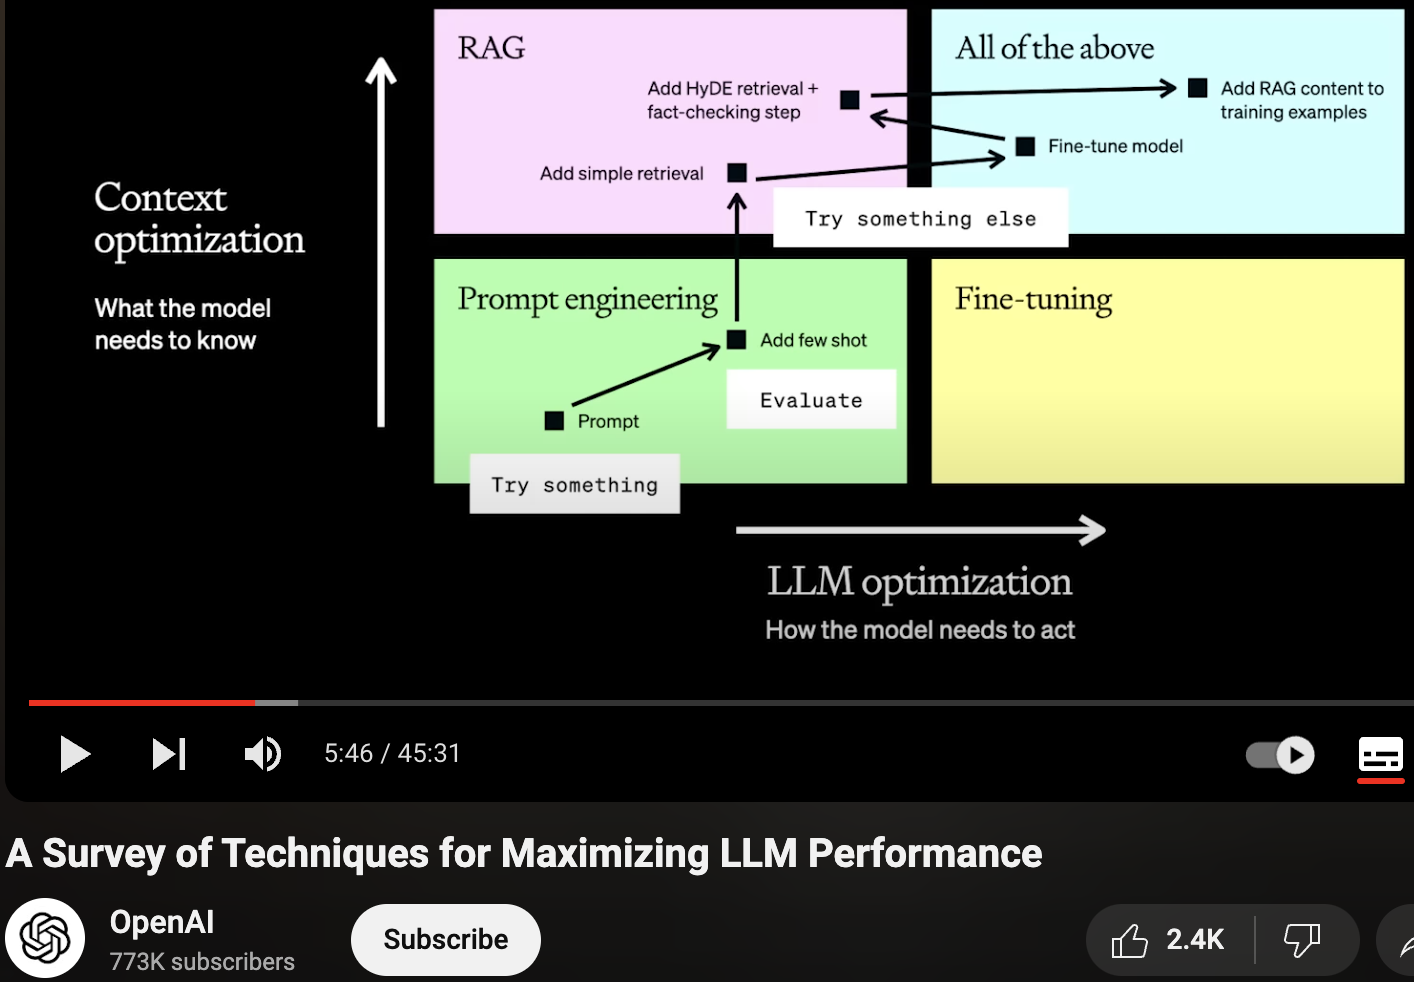
\includegraphics[width = 9cm]{figure/openai,llm,optimization.png}
\end{figure}

%\begin{itemize}
%	\item 
%\end{itemize}



\vfill

\end{vbframe}

\begin{vbframe}{RLHF lecture}

\vfill

\textbf{Roadmap}

	\begin{itemize}
		\item Motivation: Why LLM optimization?
		\item Prompt engineering
                \item Beyond prompt engineering
                  \item Exercise
                  \item More details on prompt engineering
	\end{itemize}

\vfill

\end{vbframe}



\section{Prompt engineering}

\begin{vbframe}{Prompt engineering}

\vfill

\textbf{Six strategies}


\begin{itemize}
\item
\textbf{\href{https://platform.openai.com/docs/guides/prompt-engineering/six-strategies-for-getting-better-results}{\beamergotobutton{OpenAI
prompt engineering guide}}}
	\item Write clear instructions
	\item Provide reference text
	\item Split complex tasks into simpler subtasks
        
	\item Give the model time to ``think''
        
	\item Use external tools
        
	\item Test changes systematically

\end{itemize}



\vfill

\end{vbframe}

\begin{vbframe}{Prompt engineering}

\vfill

\textbf{Strategy 1: Write clear instructions}


\begin{itemize}

\item     Include details in your query to get more relevant
    answers
\item         Ask the model to adopt a persona (e.g., be an expert)
\item             Use delimiters to clearly indicate distinct
    parts of the input
\item         Specify the steps required to complete a task
\item             Provide examples
\item                 Specify the desired length and format of the output

\end{itemize}

\vfill

\end{vbframe}

\begin{vbframe}{Prompt engineering}

\vfill

\textbf{Strategy 2: Provide reference text}


\begin{itemize}
\item (purpose: reduce hallucinations)
\item     Instruct the model to answer using a reference text
\item         Instruct the model to answer with citations from a
        reference text

\end{itemize}

\vfill

\end{vbframe}
\begin{vbframe}{Prompt engineering}

\vfill

\textbf{Strategy 3: Split complex tasks into simpler subtasks}


\begin{itemize}

\item (it's much easier for the model to answer simple tasks
and then stitch together the results than answer a  complex task)
\item     Use intent classification to identify the most relevant
    instructions for a user query
\item         For dialog applications that require very long
    conversations, summarize or filter previous dialog
\item         Summarize long documents piecewise and construct a
    full summary recursively

\end{itemize}

\vfill

\end{vbframe}
\begin{vbframe}{Prompt engineering}

\vfill

\textbf{Strategy 4: Give the model time to ``think''}


\begin{itemize}

\item (e.g., chain of thought)
\item     Instruct the model to work out its own solution before
    rushing to a conclusion
\item         Use inner monolog or a sequence of queries to hide
    the model's reasoning process
\item         Ask the model if it missed anything on previous passes

\end{itemize}

\vfill

\end{vbframe}


\begin{vbframe}{Prompt engineering}

\vfill

\textbf{Strategy 5: Use external tools}


\begin{itemize}


\item     Use embedding-based search to implement efficient
    knowledge retrieval, e.g., RAG
\item         Use code execution to perform more accurate
    calculations or call external APIs
\item         Give the model access to specific functions

\end{itemize}

\vfill

\end{vbframe}
\begin{vbframe}{Prompt engineering}

\vfill

\textbf{Strategy 6: Test changes systematically}


\begin{itemize}
\item (it's hard/impossible to assess changes based on
anecdotal evidence)
\item     Evaluate model outputs with reference to gold-standard answers

\end{itemize}

\vfill

\end{vbframe}


\begin{vbframe}{RLHF lecture}

\vfill

\textbf{Roadmap}

	\begin{itemize}
		\item Motivation: Why LLM optimization?
		\item Prompt engineering
                \item Beyond prompt engineering
                  \item Exercise
                  \item More details on prompt engineering
	\end{itemize}

\vfill

\end{vbframe}



\section{Beyond prompt engineering}




\begin{vbframe}{System message}

\vfill

\textbf{Ways we can exploit the system message}

	\begin{itemize}
		\item Generally: helps set the assistant's
		behavior
		\item Give the model general instructions
		that should govern its global behavior
		(e.g., 3H)
                		\item Give the assistant a persona
                \item Give the model a summary of a long context
                \item Instruct the model to check its own output
\item For calculations: always generate and then execute code
	\end{itemize}

\vfill

\end{vbframe}


\begin{vbframe}{Doubts about LLM optimization}

\vfill

\textbf{What is the halflife of this lecture?}

	\begin{itemize}
		\item ``I've been hesitant lately to dedicate a lot of time to
learning how to perfect prompts. It appears every new
version, not to mention different LLMs, responds
differently. With the rapid advancement we're seeing, in two
years or five, we might not even need such complex prompting
as systems get smarter.''
\item https://www.infoq.com/news/2023/12/openai-prompt-engineering/
\item (apart from systems getting smarter, their very nature
may also change rapidly as has been the case in the last 2-5
		years)
	\end{itemize}

\vfill

\end{vbframe}

\begin{vbframe}{RLHF lecture}

\vfill

\textbf{Roadmap}

	\begin{itemize}
		\item Motivation: Why LLM optimization?
		\item Prompt engineering
                \item Beyond prompt engineering
                  \item Exercise
                  \item More details on prompt engineering
	\end{itemize}

\vfill

\end{vbframe}


\section{Exercise}

\begin{vbframe}{Exercise}

\vfill

\textbf{Information extraction task}

\begin{itemize}
                \item Given: a sentence, e.g., ``After
                working as a carpenter after school, Mary now has
                been with BMW for 10 years.''
\item Output: (Mary,is-employed-by,BMW)
\item There is a small set of four relations: is-employed-by,
                reports-to,
                his/her-job-role-is, his/her-degree-is
\item Optimize LLM performance for this task
\item Work in groups!

\end{itemize}

\vfill

\end{vbframe}


\begin{vbframe}{RLHF lecture}

\vfill

\textbf{Roadmap}

	\begin{itemize}
		\item Motivation: Why LLM optimization?
		\item Prompt engineering
                \item Beyond prompt engineering
                  \item Exercise
                  \item More details on prompt engineering
	\end{itemize}

\vfill

\end{vbframe}


\section{More details on prompt engineering}

\begin{vbframe}{}

\vfill


\href{https://platform.openai.com/docs/guides/prompt-engineering}{\beamergotobutton{OpenAI Prompt Engineering Guide}}



\vfill

\end{vbframe}


\endlecture
\end{document}
